\clearpage
\section{Results}\label{sec:results}
\subsection{Model comparison}
Table~\ref{tab:testmetrics} compares all five pipelines on the same 25,000 test
reviews. DistilBERT + LoRA records the highest accuracy, precision, recall, F1
and ROC-AUC. TF-IDF + LinearSVC is the strongest classical baseline.

\begin{table}[htbp]\centering\small
\caption{Test performance (positive class = 1). Metrics are fractions; LR means Logistic Regression. ROC-AUC is a ranking measure.}\label{tab:testmetrics}
\begin{tabular}{@{}lrrrrr@{}}\toprule
Pipeline & Accuracy & Precision & Recall & F1 & ROC-AUC\\\midrule
\tableinput{tables/test_metrics.tex}
\bottomrule\end{tabular}
\end{table}

The exact accuracy improvement over TF-IDF + LinearSVC is
$0.92564-0.88684=0.03880$, or 3.880 percentage points. F1 improves by 0.0403
when rounded to four decimal places. DistilBERT makes 1,859 errors compared
with 2,829, a reduction of 970 errors or approximately 34.3\% relative to that
baseline. These are observed differences, without a multi-seed uncertainty
estimate or a claim that architecture alone caused the gain.

\begin{table}[htbp]\centering\small
\caption{Recorded validation metrics. The DL row is the selected checkpoint of the final retraining run, not the search-run maximum.}\label{tab:valmetrics}
\begin{tabular}{@{}lrrrr@{}}\toprule
Pipeline & Accuracy & Precision & Recall & F1\\\midrule
\tableinput{tables/validation_metrics.tex}
\bottomrule\end{tabular}
\end{table}

\subsection{Representation and classifier effects}
TF-IDF outperforms averaged Word2Vec with both classifiers: the accuracy advantage
is 2.408 percentage points with LR and 2.964 points with LinearSVC. Within the
TF-IDF branch, switching LR to LinearSVC raises accuracy by 0.648 points; within
Word2Vec, the change is only 0.092 points. For these configurations, the choice
of representation has a larger effect than the choice between the two linear
classifiers. Figure~\ref{fig:mlscores} shows the same classical comparison.

TF-IDF's lexical and bigram evidence is useful for review polarity. The mean
Word2Vec vector can express distributional similarity, but its pooling discards
order and treats sentiment-bearing phrases as contributions to one average.
The results support TF-IDF over this particular Word2Vec setup; they do not
establish that every embedding method is inferior. Similarly, the deep model
benefits from pretrained contextual knowledge, different input preparation and
more tuning, so its gain is a whole-pipeline result.

\reportfigure{person2_image3.png}{0.92}{Test accuracy and F1 of our four classical pipelines. The vertical axis begins at 80\%, emphasizing differences among the pipelines.}{fig:mlscores}

\subsection{Confusion matrices and error direction}
Table~\ref{tab:confusions} gives the exact counts behind the required metrics.
Figure~\ref{fig:confusions} shows our confusion matrices in two panels so that
labels remain readable.
Within each matrix, percentages are relative to the true class, whose size is
12,500.

\begin{table}[htbp]\centering\small
\caption{Test confusion counts. Negative is class 0; positive is class 1.}\label{tab:confusions}
\begin{tabular}{@{}lrrrrr@{}}\toprule
Pipeline & TN & FP & FN & TP & Errors\\\midrule
\tableinput{tables/confusion_counts.tex}
\bottomrule\end{tabular}
\end{table}

\begin{figure}[htbp]\centering
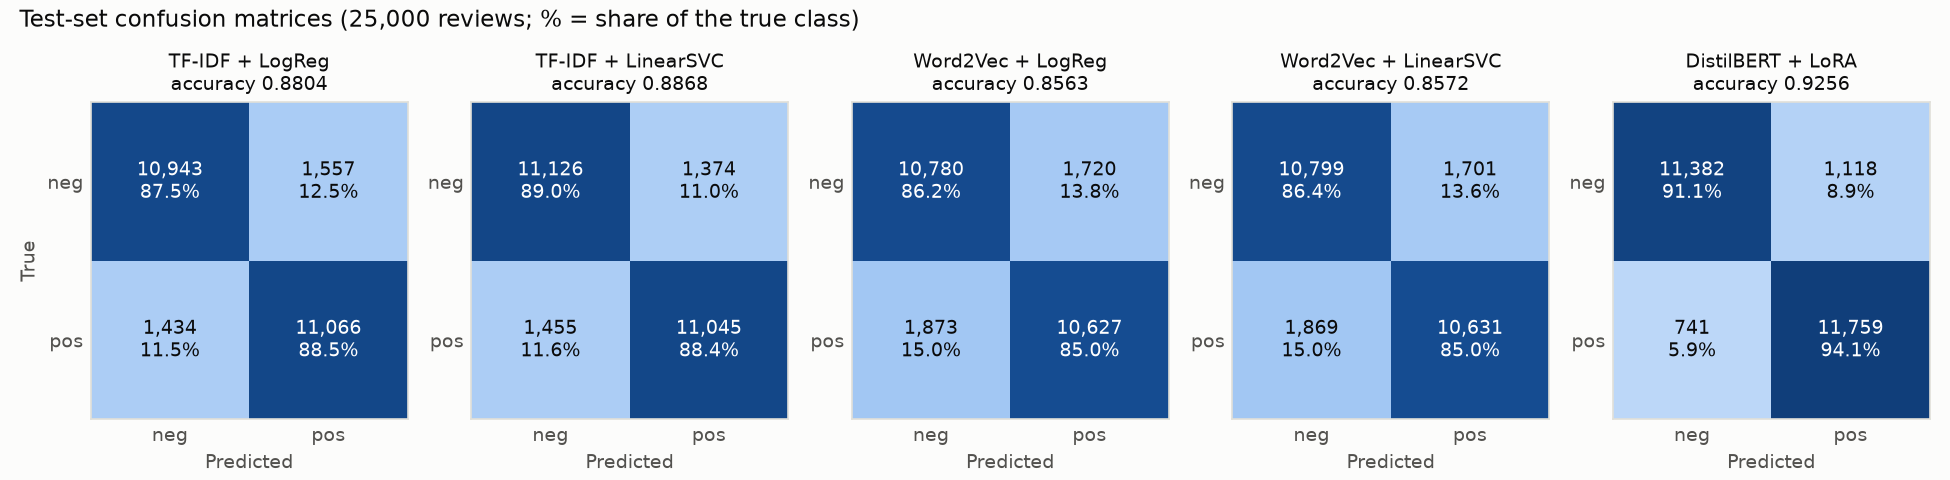
\includegraphics[width=\linewidth,trim=0 0 374.37bp 0,clip]{assets/report/person4_rId23.png}\\[5mm]
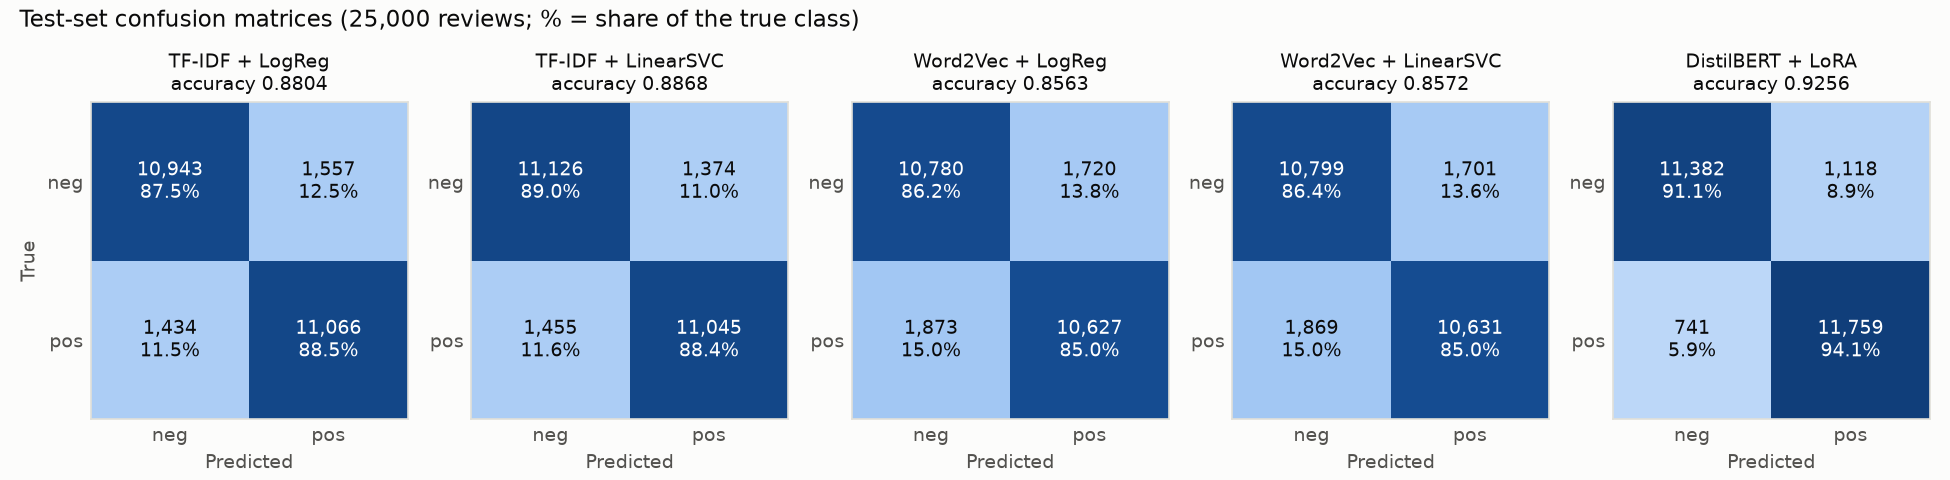
\includegraphics[width=0.68\linewidth,trim=561.55bp 0 0 0,clip]{assets/report/person4_rId23.png}
\caption{Test confusion matrices for the five pipelines. Upper panel: TF-IDF + LR, TF-IDF + LinearSVC, Word2Vec + LR. Lower panel: Word2Vec + LinearSVC, DistilBERT + LoRA. Rows are true labels; columns are predictions.}
\label{fig:confusions}
\end{figure}

DistilBERT has 1,118 false positives and 741 false negatives. It retrieves
94.072\% of positive reviews but incorrectly marks 8.944\% of negative reviews
as positive. This positive prediction tendency explains recall exceeding
precision. TF-IDF + LinearSVC is more balanced, with 1,374 false positives and
1,455 false negatives. Our cross-model analysis finds 708 test rows
wrong for all five pipelines, or 702 after exact-text deduplication. Shared
errors motivate the stratified analysis in Section~\ref{sec:errors}.

\subsection{Recorded computational cost}
The saved classical classifier-fit times are 1.092 s (TF-IDF + LR), 0.309 s
(TF-IDF + LinearSVC), 0.077 s (Word2Vec + LR), and 0.282 s (Word2Vec + LinearSVC).
These timers wrap classifier fitting only: they exclude TF-IDF construction,
Word2Vec training, document pooling and preprocessing. Hardware and timing scope
also differ from the GPU run, so these figures are not end-to-end speed ratios.

The final DistilBERT run records 2,004.80 s of training across ten epochs,
excluding validation passes, with approximately 200 s per epoch at length 512.
The eight-run search records approximately 9,998 s of training in total.
Peak allocated GPU memory is approximately 2,911 MiB. LoRA limits optimized
parameters to 739,586 relative to the 66,955,010 base-model reference count,
but these records do not include a full-fine-tuning baseline and therefore do
not quantify a measured speedup over full fine-tuning.
\FloatBarrier
